% Copyright (c) 2026 IBM
%
% Must be processed with XeLaTeX

% Local Variables:
% coding: utf-8
% End:

\documentclass[xetex, table, 10pt,%
aspectratio=169%
]{beamer}
\usepackage{fontspec}
\usepackage{array}
\usepackage{tabularx}
\usepackage{colortbl}
\usepackage{wasysym}
\usepackage{hyperref}
\usepackage{graphicx}
\usepackage{textcomp}

\usepackage[english]{babel}

\usepackage{tikz}
\usepackage{pifont}
\usetikzlibrary{shapes}
\usetikzlibrary{positioning}
\usetikzlibrary{fit}
\usetikzlibrary{arrows}
\usetikzlibrary{decorations.pathreplacing}
\usetikzlibrary{decorations.pathmorphing}
\usetikzlibrary{shadows}
\usetikzlibrary{shapes.symbols}
\usetikzlibrary{shapes.callouts}
\usetikzlibrary{chains}
\usetikzlibrary{patterns}

\usetheme{ClearIBM}
\setmainfont{IBM Plex Serif}
\setsansfont{IBM Plex Sans}
\setmonofont{IBM Plex Mono}

\newfontfamily\symbolfont{DejaVu Sans}
\beamertemplatenavigationsymbolsempty

\hypersetup{
  pdftitle={Paravirt Scheduling: Framework for better CPU usage},
  pdfauthor={Shrikanth Hegde, Ilya Leoshkevich},
  pdfsubject={OSPM 2026},
  pdfkeywords={paravirt, scheduling, vCPU},
  pdfstartview=Fit,
  colorlinks=true,
  urlcolor=blue,
  linkcolor=black}

\title[Paravirt Scheduling]{Paravirt Scheduling:\\ Framework for better CPU usage}
\author{Shrikanth Hegde \and Ilya Leoshkevich}
\institute{IBM}
\date{OSPM 2026, Cambridge}

\pgfdeclarelayer{background}
\pgfdeclarelayer{foreground}
\pgfsetlayers{background,main,foreground}

\begin{document}

\frame[plain]{\titlepage}

\begin{frame}{Agenda}
\begin{itemize}
  \item Problem Statement and proposed Solution
  \item Existing methods
  \item Journey so far
  \item Design goals
  \item Implementation details
  \item s390 background
  \item Performance numbers
  \item Open questions
\end{itemize}
\end{frame}

\section{Problem Statement and Solution}

\begin{frame}{Problem Statement: vCPU Overcommit and vCPU Preemption}
\begin{columns}
\column{0.55\linewidth}
\begin{itemize}
  \item Multiple VMs sharing the underlying CPU resources, with
    overcommit (sum of vCPUs $>$ pCPUs)
  \item High CPU utilization in multiple VMs at the same time leads
    to vCPU preemption
  \item Why vCPU preemption can be expensive:
  \begin{itemize}
    \item \textbf{vCPU context:} a vCPU may be holding a mutex or
      spinlock
    \item \textbf{Hypervisor overhead:} hypervisors may schedule at a
      different granularity than the guest, introducing extra delays
      and cache/TLB thrashing on vCPU migration
  \end{itemize}
  \item \textbf{Design constraint:} the hypervisor is
    non-cooperative -- no host-side changes,
    no inter-guest channel (e.g.\ PR/SM, PowerVM)
\end{itemize}
\column{0.45\linewidth}
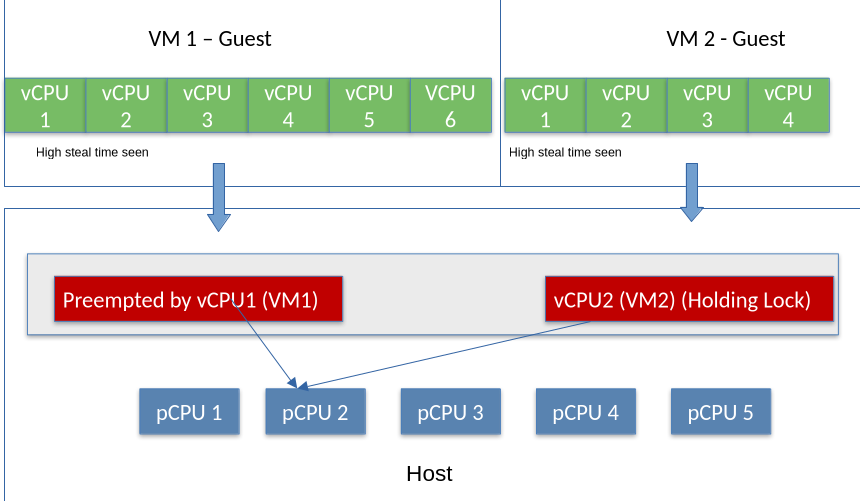
\includegraphics[width=\linewidth]{problem}
\end{columns}
\end{frame}

\begin{frame}{Proposed Solution: steal-driven vCPU backoff}
\begin{columns}
\column{0.55\linewidth}
\begin{itemize}
  \item The vCPUs each guest can safely use are denoted as
    \emph{preferred} CPUs
  \item \textbf{Aim:} sum of preferred CPUs $\le$ pCPUs, which
    achieves less vCPU preemption
  \item \textbf{Mechanism:} each guest independently adjusts its
    preferred CPU set from locally observed steal time
  \item \textbf{Fairness:} all guests run the same backoff logic, so
    they converge without talking to each other
\end{itemize}
\medskip
Advantage of a context switch within the vCPU instead:
\begin{itemize}
  \item Lockholder runs to completion (\texttt{preempt\_disable()})
  \item No hypervisor overhead
\end{itemize}
\column{0.45\linewidth}
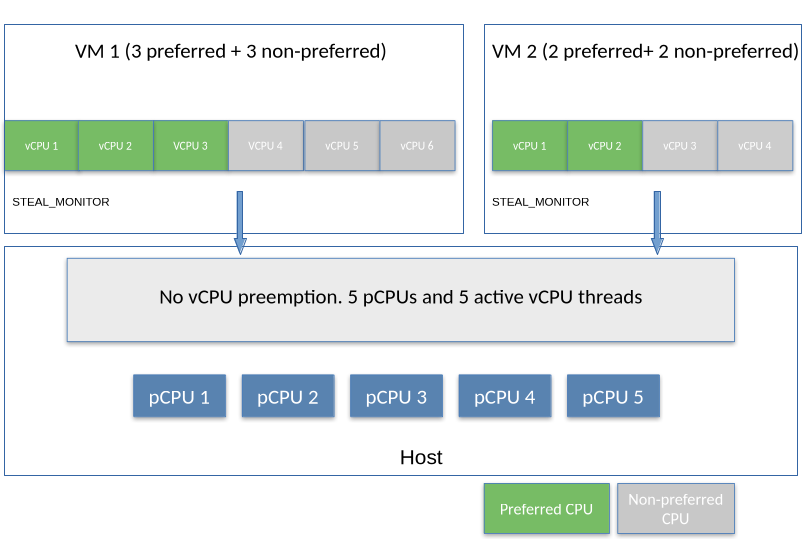
\includegraphics[width=\linewidth]{solution}
\end{columns}
\end{frame}

\section{Existing methods}

\begin{frame}{Existing Methods}
Discussed in detail at LPC 2025 -- why no existing methods work.
A quick glance:
\begin{itemize}
  \item \textbf{Explicit affinity:} can't expect a user to set
    affinity for each workload
  \item \textbf{CPU hotplug:} slow, expensive, breaks user-specified
    affinities
  \item \textbf{Isolated cpuset partitions:} needs sched domain
    rebuild, breaks user-specified affinities
  \item \textbf{Capacity-aware scheduling:} doesn't push tasks from a
    CPU under high load
\end{itemize}
\end{frame}

\section{Journey so far}

\begin{frame}{Journey so far\ldots}
\begin{itemize}
  \item \textbf{LPC 2024} -- introduced the problem statement. A new
    load balancing type \texttt{cpu\_parked} was used. This was a
    PoC, slow in moving tasks since it depended on the load balancer
    and heavily on stats.\\
    {\small\href{https://lore.kernel.org/all/20241204112149.25872-1-huschle@linux.ibm.com/\#r}{[RFC
    PATCH 0/2] sched/fair: introduce new scheduler group type
    \texttt{group\_parked}}}
  \item \textbf{LPC 2025:} a few revisions later, switched to a
    push-task-mechanism-based method. Much faster and more
    policy-driven than stats.\\
    {\small\href{https://lore.kernel.org/all/20251119124449.1149616-1-sshegde@linux.ibm.com/\#r}{[PATCH
    00/17] Paravirt CPUs and push task for less vCPU preemption}}
\end{itemize}
\end{frame}

\section{Design goals}

\begin{frame}{Design Goals}
\begin{itemize}
  \item Keep runnable vCPUs close to pCPU count under contention
  \item Preserve user-specified CPU affinity
  \item Keep the solution scheduler-native and lightweight
  \item Provide a debug tunable to adjust based on the platform
  \item Expose the new CPU state information for consumption
  \item Do not preclude future hypervisor-assisted solutions
\end{itemize}
\end{frame}

\section{Implementation details}

\begin{frame}{New CPU State: \texttt{cpu\_preferred\_mask}}
\begin{itemize}
  \item Represents CPUs the scheduler should currently prefer
  \item Not a hard exclusion: affinity is still respected
  \item Dynamic and policy-driven
  \item Maintains the design construct:\\
    preferred $\subseteq$ online $\subseteq$ possible
\end{itemize}
\end{frame}

\begin{frame}{Sched feature: \texttt{STEAL\_MONITOR}}
\begin{itemize}
  \item In \texttt{sched\_tick()}, check if it is time to compute steal
    time
  \item Kick off a work function to compute steal time -- keeps
    \texttt{sched\_tick()} latency minimally affected
  \item Compute steal time ratio from \texttt{CPUTIME\_STEAL} across
    all online CPUs
  \item If steal time is above the threshold, reduce preferred CPUs
  \begin{itemize}
    \item Current implementation reduces by one core, because some
      hypervisors (e.g.\ PowerVM) schedule at core granularity --
      this yields the best benefit
  \end{itemize}
  \item If steal time is below the threshold, increase preferred
    CPUs
  \item Simple heuristics avoid oscillations: only consecutive
    high/low steal values are considered
\end{itemize}
\end{frame}

\begin{frame}{Core APIs being updated}
\begin{itemize}
  \item \texttt{is\_cpu\_allowed()}
  \begin{itemize}
    \item Try to select a preferred CPU
    \item If task affinity is only on non-preferred CPUs, return a
      non-preferred CPU
    \item Ensure overhead is minimal for the majority use case
    \item Used by \texttt{select\_fallback\_rq()}, the push-task
      mechanism, and wake-ups
  \end{itemize}
  \item \texttt{available\_idle\_cpu()}
  \begin{itemize}
    \item Make the CPU available if it is part of preferred CPUs
    \item Handles wake-up decisions; used by CFS
  \end{itemize}
  \item \texttt{\_\_cpupri\_find()}
  \begin{itemize}
    \item Consider only preferred CPUs when finding
      \texttt{lowest\_rq} for RT tasks
  \end{itemize}
\end{itemize}
\end{frame}

\begin{frame}{How it all fits together}
\begin{itemize}
  \item On task wake-up, when choosing a CPU, pick a preferred CPU
    where possible
  \item Load-balance only among preferred CPUs, so load balance and
    push-task don't fight each other; load stays on preferred CPUs
  \item At \texttt{sched\_tick()}, the first check: is this CPU
    non-preferred? If so, push the task out via a stopper thread.
    Only the current task is pushed (keeps it simple). Since the
    work is not done in \texttt{sched\_tick()}, IRQ latency shouldn't
    increase much
  \item A task is pushed only if it doesn't break affinity. If a
    task is bound only on non-preferred CPUs, there is no point
    pushing it out
\end{itemize}
\medskip
{\small\href{https://lore.kernel.org/all/20260407191950.643549-1-sshegde@linux.ibm.com/\#r}{[PATCH
v2 00/17] sched/paravirt: Introduce \texttt{cpu\_preferred\_mask} and
steal-driven vCPU backoff}}
\end{frame}

\begin{frame}[fragile]{User Visibility \& Control}
\begin{itemize}
  \item \texttt{/sys/devices/system/cpu/preferred} -- current
    preferred CPUs
  \item \texttt{STEAL\_MONITOR} sched feature
  \item Debugfs knobs for thresholds and sampling period -- escape
    hatch for debugging, not a per-workload admin interface
  \item Plan: pick per-architecture defaults
\end{itemize}
\begin{verbatim}
# echo STEAL_MONITOR > /sys/kernel/debug/sched/features
# echo NO_STEAL_MONITOR > /sys/kernel/debug/sched/features

# pwd
/sys/kernel/debug/sched
steal_mon_high:500
steal_mon_low:200
steal_mon_period:1000
\end{verbatim}
\end{frame}

\section{s390 background}

\begin{frame}{s390 challenges}
\begin{itemize}
  \item Large system: \textasciitilde 200 cores
  \item There is no bare-metal Linux on s390
  \item Proprietary type-1 hypervisor: PR/SM
  \begin{itemize}
    \item Unlikely to add Linux-specific enhancements
  \end{itemize}
  \item Overcommit and steal time
  \item Whole-system performance vs.\ single-VM performance
\end{itemize}
\end{frame}

\begin{frame}{s390 Hiperdispatch}
\begin{itemize}
  \item PR/SM designates CPUs as high, medium, and low, and lets the
    guest know which is which
  \item PR/SM frequently steals low CPUs for a long time
  \item Problem: exits to PR/SM are expensive
  \item Idea: avoid scheduling threads on low CPUs that had steal
    time recently
\end{itemize}
\medskip
\textbf{Hiperdispatch}
\begin{itemize}
  \item Created by Tobias Huschle and Mete Durlu
  \item Upstream since v6.12
  \item Uses capacity-aware scheduling
  \item Does not handle heavy overcommit
\end{itemize}
\end{frame}

\begin{frame}{s390 Warning Track Interrupt}
\begin{itemize}
  \item Problem: contention if a lock holder is stolen
  \item PR/SM sends an interrupt shortly before stealing a CPU
  \item Idea: park CPUs that are about to be stolen to prevent them
    from taking locks
\end{itemize}
\medskip
\textbf{WTI}
\begin{itemize}
  \item Created by Tobias Huschle and Mete Durlu
  \item Upstream since v6.12
  \item Schedules a real-time thread to yield to the hypervisor ASAP
\end{itemize}
\end{frame}

\section{Performance numbers}

\begin{frame}{Performance numbers: PowerPC / PowerVM hypervisor}
\begin{center}
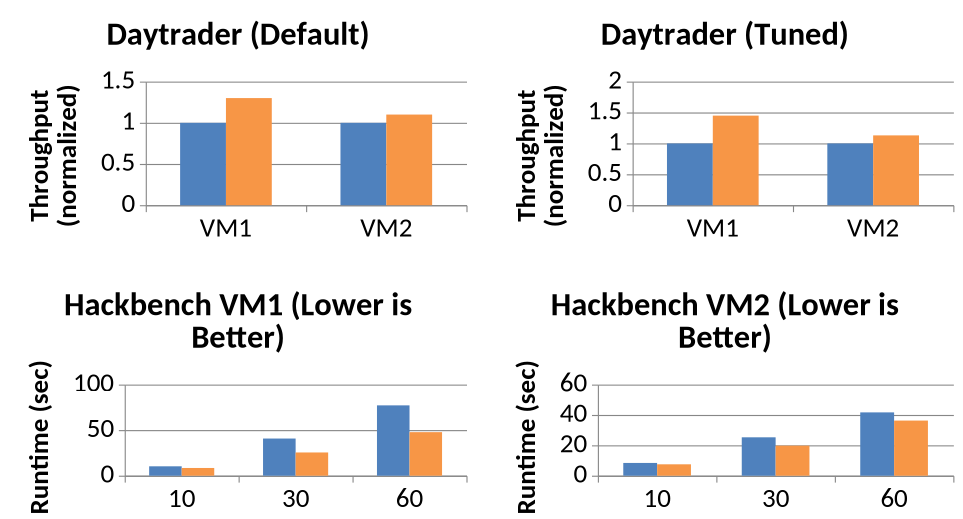
\includegraphics[width=0.85\linewidth,height=0.75\textheight,keepaspectratio]{perf-powerpc}
\end{center}
\end{frame}

\begin{frame}{Performance numbers: s390 PR/SM}
\begin{itemize}
  \item s390 host with 37 cores
  \item 4 partitions with 37 shared cores each
  \item Workload 1: \texttt{stress-ng -{}-matrix 37}
  \item Workload 2: \texttt{uperf} ping-pong
  \item Workload 3: \texttt{uperf} streaming
\end{itemize}
\medskip
\textbf{Results:}
\begin{itemize}
  \item \textasciitilde 2x throughput improvement for all workloads
  \item Steal time reduction from \textasciitilde 60\% to
    \textasciitilde 5\%
\end{itemize}
\end{frame}

\begin{frame}{Performance numbers: KVM}
\begin{itemize}
  \item 2--16 VMs
  \item 4--32 CPUs each
  \item s390 host with 16 cores
  \item x86\_64 host with 32 cores
  \item Up to 4x overcommit
  \item Each VM runs the same benchmark
  \begin{itemize}
    \item \texttt{hackbench}, \texttt{pgbench}, \texttt{schbench},
      \texttt{sysbench}
  \end{itemize}
  \item Throughputs are summed across all VMs
  \item Repeated 10 times to quantify noise
\end{itemize}
\end{frame}

\begin{frame}{Performance numbers: s390 KVM}
\vspace*{-0.8cm}
\begin{center}
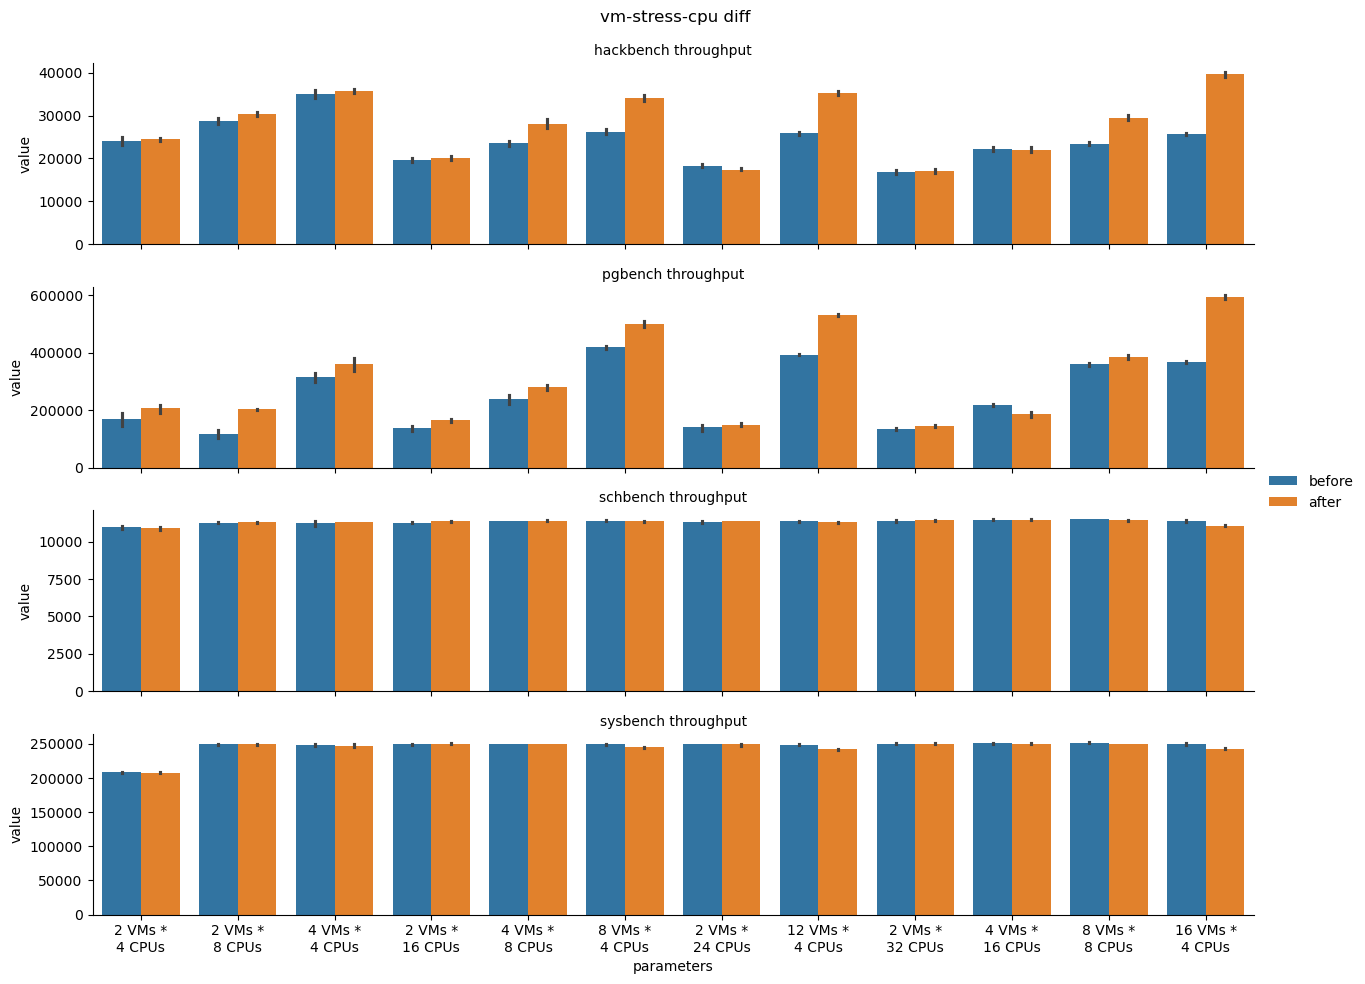
\includegraphics[width=0.92\paperwidth,height=0.92\paperheight,keepaspectratio]{perf-s390-kvm}
\end{center}
\end{frame}

\begin{frame}{Performance numbers: x86\_64 KVM}
\vspace*{-0.8cm}
\begin{center}
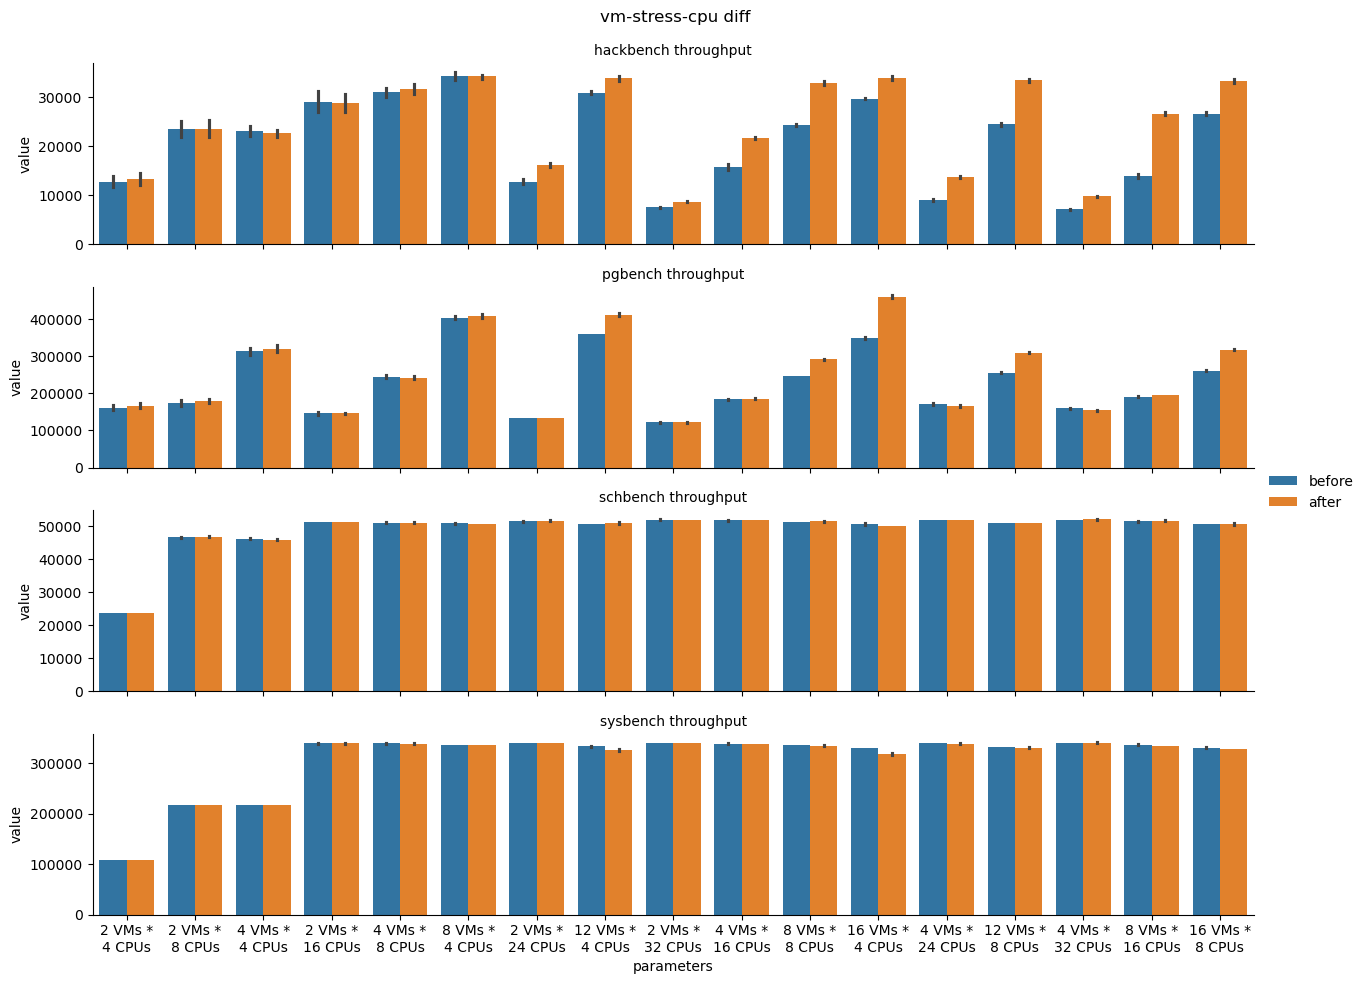
\includegraphics[width=0.92\paperwidth,height=0.92\paperheight,keepaspectratio]{perf-x86-kvm}
\end{center}
\end{frame}

\section{Open questions}

\begin{frame}{Open Questions: Concept}
\begin{itemize}
  \item Is the design sound for the majority use case?
  \item Upstream readiness?
  \item Is there any !SMT system interested in this?
  \item How to avoid oscillations in complex overcommit cases?
  \item \texttt{irqbalance} must be made preferred-mask-aware; when
    it is off, should the kernel push IRQs off non-preferred CPUs?
  \item Should \texttt{sched\_ext} tasks be pushed too, in addition to
    the fair and RT tasks handled today?
\end{itemize}
\end{frame}

\begin{frame}{Open Questions: Implementation}
\begin{itemize}
  \item Arch-specific hook to choose which CPU to drop from the
    preferred mask, e.g.\ based on power entitlements or s390
    polarization
  \begin{itemize}
    \item Default: NUMA-aware -- pack onto one node, or spread
      across nodes? Spreading likely wins -- more resources overall
      at the cost of cross-node penalties
  \end{itemize}
  \item \texttt{STEAL\_MONITOR} off by default, with each arch
    opting in -- is that the right default?
\end{itemize}
\end{frame}

\section*{Backup}

\begin{frame}{Backup: avoiding host under-utilization}
\begin{itemize}
  \item \textbf{Implemented today:} fast shrink, slow grow -- same
    as TCP
  \item \textbf{Idea:} EWMA-filter the steal time signal -- same
    as PELT
  \item \textbf{Idea:} rate limit preferred-mask changes
  \item \textbf{Idea:} randomize the sampling phase and mask-change
    rate across guests to avoid synchronized decisions
\end{itemize}
\end{frame}

\begin{frame}{Backup: fairness without coordination}
\begin{itemize}
  \item Non-cooperative hypervisors are the main reason this work
    exists
  \item Coordination via the host is not an option on PR/SM or PowerVM
  \item Similar to TCP: no central coordinator
  \item One could do better there with explicit host cooperation, but
    the uncoordinated mechanism already improves things
\end{itemize}
\end{frame}

\begin{frame}{Backup: is this SMT-specific?}
\begin{itemize}
  \item No. Nothing in the mechanism depends on SMT
  \item Current implementation adjusts the preferred mask by one
    \emph{core} only because some hypervisors (e.g.\ PowerVM) schedule
    at core granularity
\end{itemize}
\end{frame}

\begin{frame}{Backup: steal time collection context}
\begin{itemize}
  \item Under heavy overcommit the kworker itself can be stolen
  \item \textbf{Idea:} keep the computation inside the tick
  \item Precedent: PELT already runs inline from the tick, so this
    would not be worse:\\
    \texttt{sched\_tick() $\to$ task\_tick\_fair() $\to$
    entity\_tick() $\to$ update\_load\_avg() $\to$
    \_\_update\_load\_avg\_se()}
\end{itemize}
\end{frame}

\begin{frame}{Backup: relative steal time}
\begin{itemize}
  \item Many VMs with low utilization can cause overcommit
  \item Absolute steal time misses this
  \item \textbf{Idea:} divide steal time by non-idle time
\end{itemize}
\end{frame}

\begin{frame}{Backup: replacing \texttt{stop\_one\_cpu\_nowait()}}
\begin{itemize}
  \item Current v2 pushes tasks off non-preferred CPUs via the CPU
    stopper -- heavy-handed (runs at \texttt{stop\_sched\_class},
    above RT/DL) for what is a soft placement hint
  \item \textbf{Idea:} build on Vincent Guittot's CFS push-task mechanism
  \item {\small\href{https://lore.kernel.org/all/20251202181242.1536213-1-vincent.guittot@linaro.org/}{[PATCH
    0/6 v8] sched/fair: Add push task mechanism and handle more EAS
    cases}}
  \item \textbf{Idea:} extend it to push all tasks off a CPU
  \item \textbf{Idea:} reuse the CPU-offline task pushing code
\end{itemize}
\end{frame}

\begin{frame}{Legal statement}
\begin{itemize}
  \item This work represents the view of the authors and does not
    necessarily represent the view of IBM
  \item IBM and IBM (logo) are trademarks or registered trademarks
    of International Business Machines Corporation in the United
    States and/or other countries
  \item Linux is a registered trademark of Linus Torvalds
  \item Other company, product, and service names may be trademarks
    or service marks of others
\end{itemize}
\end{frame}

\begin{frame}[plain]
\begin{center}
{\Huge Thank You}
\end{center}
\end{frame}

\end{document}
